\documentclass{acm_proc_article-sp}

\usepackage{url, hyperref}

\begin{document}

\title{Spatial Data Indexing Using Grid-Based Method and KD-Tree Method\titlenote{This report is intended to be the final report of \textit{Spatial-Temporal Data Analysis}, which is a class lectured by Professor \textit{Zheng Yu} in the summer of 2014.}}

%
% You need the command \numberofauthors to handle the 'placement
% and alignment' of the authors beneath the title.
%
% For aesthetic reasons, we recommend 'three authors at a time'
% i.e. three 'name/affiliation blocks' be placed beneath the title.
%
% NOTE: You are NOT restricted in how many 'rows' of
% "name/affiliations" may appear. We just ask that you restrict
% the number of 'columns' to three.
%
% Because of the available 'opening page real-estate'
% we ask you to refrain from putting more than six authors
% (two rows with three columns) beneath the article title.
% More than six makes the first-page appear very cluttered indeed.
%
% Use the \alignauthor commands to handle the names
% and affiliations for an 'aesthetic maximum' of six authors.
% Add names, affiliations, addresses for
% the seventh etc. author(s) as the argument for the
% \additionalauthors command.
% These 'additional authors' will be output/set for you
% without further effort on your part as the last section in
% the body of your article BEFORE References or any Appendices.

\numberofauthors{1} %  in this sample file, there are a *total*
% of EIGHT authors. SIX appear on the 'first-page' (for formatting
% reasons) and the remaining two appear in the \additionalauthors section.
%
\author{
% You can go ahead and credit any number of authors here,
% e.g. one 'row of three' or two rows (consisting of one row of three
% and a second row of one, two or three).
%
% The command \alignauthor (no curly braces needed) should
% precede each author name, affiliation/snail-mail address and
% e-mail address. Additionally, tag each line of
% affiliation/address with \affaddr, and tag the
% e-mail address with \email.
%
% 1st. author
\alignauthor
Kaichun Mo\titlenote{I'm a undergraduate student from ACM Honered Class, SJTU, majoring in CS. }\\
       \affaddr{ACM Honered Class, SJTU}\\
       \affaddr{Shanghai, China}\\
       \email{daerduoCarey@163.com}
}
% There's nothing stopping you putting the seventh, eighth, etc.
% author on the opening page (as the 'third row') but we ask,
% for aesthetic reasons that you place these 'additional authors'
% in the \additional authors block, viz.
\additionalauthors{Additional authors: John Smith (The Th{\o}rv{\"a}ld Group,
email: {\texttt{jsmith@affiliation.org}}) and Julius P.~Kumquat
(The Kumquat Consortium, email: {\texttt{jpkumquat@consortium.net}}).}
\date{30 July 1999}
% Just remember to make sure that the TOTAL number of authors
% is the number that will appear on the first page PLUS the
% number that will appear in the \additionalauthors section.

\maketitle
\begin{abstract}

In this report, I will introduce you my work on spatial data indexing using Grid-Based method and KD-Tree method respectively. 

To be more specific, I write a C++ program which can successfully retrieve all POIs in any given query range(i.e.\textit{Range Query}) as well as all top-k nearest POIs regarding to any given point(i.e.\textit{KNN Query}). I implement both using two distinct methods, which are widely known as Grid-Base Method and KD-Tree Method.
\end{abstract}

% A category with the (minimum) three required fields
\category{}{Data Management}{Spatial Data Indexing}

\keywords{Spatial Data Indexing, POI, Grid-Base Method, KD-Tree Algorithm, Range Query, KNN Query} % NOT required for Proceedings
\\

\section{Introduction}

Spatial data indexing plays an indispensable role in almost all modern web service providers. All web services involved map indexing or minimum routine recommendation are pursuing efficient methods to store and index untold many POIs (Point of Interests) in the real world.

Many basic methods work pretty well, such as Grid-Based Method, which is the most intuitive method and easiest method to implement as well. But, it's apparent drawbacks definitely impede the usage of this method. More tricky but efficient methods are proposed by computer scientists. In this report, I will use KD-Tree to implement the both two kinds of queries and show you that this method does a better tradeoff between spatial complexity and temporal complexity.

In the last part of this report, I will compare the performance of the two different methods using the real data.
\\

\section{Grid-Based Method}

This section introduces the basic idea of Grid-Based method as well as the concrete implementation details involved in programming.

\subsection{Brief Introduction }

Grid-Based method is the most intuitive method to fulfill the job. The basic idea is just to divide the whole space into a bunch of grids. Each grid are considered as the basic impartible block containing a relatively small number of POIs. When encountering range query, we can just search all grids which intersect with the this range for all possible contained POIs. If a KNN query is asked, we can search the surrounding grids to the query point for the nearest $k$ POIs.

This method is easy to implement and have both pros and cons. The more specific performance analysis will be mentioned in the last part of this section.


\subsection{Algorithm Overview } 

The methods used to deal with range queries and KNN queries are quite easy. Following are the brief overviews for all methods respectively.

\subsubsection{Initialization}
\begin{itemize}
\item  Linearly scan all the POIs and figure out the smallest rectangle range that contains all POIs.
\item Divide the huge rectangle into grids and store all the grids in a list. All the POIs in one specific grid are linked sequentially.
\item Each grid can be directly accessed by some trifle computing.
\end{itemize}

\subsubsection{Rectangle Range Query}
\begin{itemize}
\item For each rectangle queried range, denotes it by left-upper point and right-bottom point.
\item Compute out all grids intersecting with this rectangle. This is easy since we can know the grid where the left-upper point lies and the gird where the right-bottom point lies. All the grids in the rectangle constituted up by this two corner grids should be involved.
\item Linearly scan all the POIs in all possible grids searching for the result.
\end{itemize}

\subsubsection{Circle Range Query}
\begin{itemize}
\item Generate the external tangent square of this queried circle.
\item Invoke the rectangle range query procedure.
\item For each grid considered, first check whether or not this grid intersects with the queried circle. If not, throw away this grid.
\end{itemize}

\subsubsection{K Nearest Neighbours Query}
\begin{itemize}
\item Figure out the grid that the point $p$ lies in, denoted as $(x,y)$, and linearly scan all POIs in it. Use a max heap to maintain the $k$ nearest POIs.
\item For each round $k=1,2,\cdots$, check all additional grids in range 
\begin{equation}
[x-k, x+k]\times [y-k, y+k]
\end{equation}
deducting 
\begin{equation}
[x-k+1, x+k-1]\times [y-k+1, y+k-1]\mbox{.}
\end{equation}
\item For each grid in the above range, if its distance to $p$ is less than the current root of the priority queue, then we linearly scan all the POIs in it and update the heap.
\item Repeat until no grid in round $k$ are scanned to update the heap.
\end{itemize}

\subsection{Performance Analysis}

This method is so intuitive that it has natural drawbacks such as ineluctable large storage required and temporal inefficiency when dealing with high unbalanced distribution of POIs. The method requires the program to store at least a pointer for each grid, which means we need to store intolerant $\Theta(\mbox{Grid Number})$ data at least. Meanwhile, if the distribution of POIs are highly unbalanced, one grid may contain too many POIs which leads to more time consuming when linearly scanning the POIs in this grid.

Notwithstanding the mortal drawbacks, the method is the easiest method to implement. Direct Accesses to a specific grid is another merits of this method.

\section{KD-Tree Method}

This is a more enlightened method to solve the possible unbalanced distribution of POIs. 

\subsection{Brief Introduction}

Using the basic Grid-Based method can perform as inefficient as possible when the distribution of POIs is unbalanced. In this case, we can use a wiser way to divide the whole range heuristically. 

\subsection{Algorithm Overview}

The methods are wiser than those of original Grid-Based method.

\subsubsection{Initialization}

\begin{itemize}
\item We build a tree-like structure to store the data. The tree looks like the following example.
\begin{center}
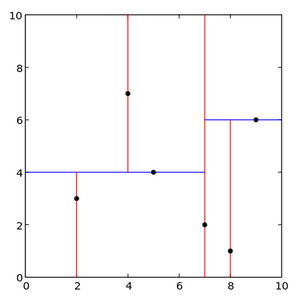
\includegraphics[width=0.2\textwidth]{pics/1.png}
\end{center}
\item Each time, we prefer to divide the POIs as balanced as possible. 
\item Each round $i$, if $i$ is even, we sort all POIs in current range with respect to the $x$ value of the points and use the middle point as the separator. If $i$ is odd, choose the separator with respect to $y$ value of the points. 
\item Now, we separate the original range into two parts. Next, we recursively invoke this procedure itself to each part, which is the procedure of round $i+1$.
\item Repeat until the current range only contain less than $m$ points, where $m$ is a given number indicating the minimum number of POIs a grid can held.
\item Note that this procedure generates a tree-like structure for us. Each interior node contains a separator point, while the leaves are indivisible grids holding a relatively small fracture of POIs.
\begin{center}
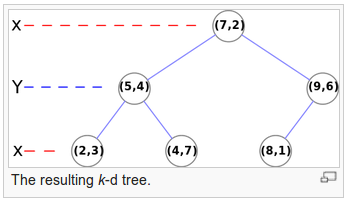
\includegraphics[width=0.3\textwidth]{pics/2.png}
\end{center}
\end{itemize}

\subsubsection{Rectangle Range Query}

\begin{itemize}
\item Start from the aspect of the root.
\item For each node we are considering, 
\begin{itemize}
\item If the node is a leaf, then linearly scan all POIs stored in this node.
\item If the queried range is separated by the separator stored in this node, we just split the queried range into two small ranges with respect to this separator and invoke this procedure itself to each part to collect more informations.
\item If the queried range lies to the left or to the right with respect to the separator POI, we just recursively invoke this procedure on the part the range lies.
\end{itemize} 
\item Repeat until all nodes are visited or cut off.
\item For each processing to one POI, just check whether or not the point is in the queried range. If the answer is yes, just add it to the final result set.
\end{itemize}

\subsubsection{Circle Range Query}

\begin{itemize}
\item Just find out the exterior tangent square of the queried circle.
\item Gather informations from the rectangle range query procedure and select the valid POIs lying in the range of the queried circle.
\end{itemize}

\subsubsection{K Nearest Neighbours Query}

\begin{itemize}
\item Start from the root of the obtained KD-Tree.
\item Maintain a max heap to store all temporary $k$ nearest POIs and guarantee that the size of this heap is by no means larger than $k$.
\item For each node visiting, we can consider this node as a rectangle range.
\begin{itemize}
\item If the node is a leaf, then just linearly scan all the POIs contained in this node and process each POI point.
\item If the node is a interior point, it must contain a separator. Use the separator to divide the current node into two small nodes. Compute the distances between each node(the corresponding rectangle) to the queried point. 
\begin{itemize}
\item If both distances are less than the worst distance in the heap, then we need to recursively invoke on each small range. We invoke the one having relatively small distance to the queried point first. 
\item If only one distance is less than the worst distance in the heap, just invoke on that viable part.
\item If both not, do nothing and quit this call of the procedure.
\end{itemize}
\end{itemize}
\item Note that there is a little trick to make this program more efficient, which is that each time we are deciding whether or not to invoke other small range, we should recheck the condition that whether or not this range's distance to queried point are less than the worst distance in the updated heap.
\item Repeat until all the nodes are visited or cut off.
\end{itemize}

\subsection{Performance Analysis}

Since the KD-Tree can deal with the situation of unbalanced distribution of POIs, we regard this method as a self-adaptive method. This property guarantees that each query is efficiently enough no matter what the inputs or the query range is.

Meanwhile, the spatial complexity is tolerable, since all the grids contain proportionable points, which means no grid is empty and wasted. This leads to the fact that this method has a dramatically less spatial complexity compared to the original Grid-Based method.

But, this method also has some drawbacks. Since the data are constructed into a tree-like structure, we can not access one node directly, which means we need more time to access one node. Besides, the implementation is relatively harder. 

\section{Performance Comparison}

Since the given data is of a small scale, so I decide to regard all POI categories as one general category. 

I adopt the following method to compute the running time.
\begin{itemize}
\item Each POI scanning accounts for ONE unit time.
\item Each main procedure invocation accounts for ONE unit time.
\item Each node or grid accounts for ONE unit time when it has been focused on.
\end{itemize}

I DO NOT take the following running time in my consideration.
\begin{itemize}
\item The time of copying a result when the copy is only needed for passing the returned value.
\begin{itemize}
\item Since the copy of returned value is just counted when counting the number of procedure invocation, counting it again seems not very necessary.
\end{itemize}
\item The time of processing general operations and comparisons.
\begin{itemize}
\item It's hard to decide how to count the running time of this part. If the data scale increases to a large extent, this part of time consuming is just a constant factor multiplied to the total time consuming.
\end{itemize}
\item The time wasted due to my lack of ability to optimize the algorithm.
\begin{itemize}
\item Actually, I can figure out some wiser way to eliminate this part of time consuming. But, in fact, I do not want to re-program due to the time limitation.
\end{itemize}
\end{itemize}

Following is the result of time consuming based on my evaluation method. (Here we assume in KD-Tree method, each leaf cannot contain more than 3 points.)

\begin{center}
\begin{tabular}{|c||c|c|c|}
\hline
\textbf{Method} & \textbf{Rec Query} & \textbf{Cir Query} & \textbf{10-NN} \\
\hline
Brute Scan & 2020 & 2020 & 2020 \\
\hline
$5\times 5$ G-B & 619 & 237 & 244 \\
\hline
$10\times 10$ G-B & 128 & 202 & 227 \\
\hline
$50\times 50$ G-B & 255 & 110 & 156 \\
\hline
KD-Tree & 101 & 117 & 68 \\
\hline
\end{tabular}
\end{center}

From the above result, we can know
\begin{itemize}
\item Using Grid-Based method, one should find a good tradeoff between too many grids and too concentrated POIs in one grid.
\item Using KD-Tree method, the result is relatively compelling and attractive.
\end{itemize}

\section{Conclusion}

In this report, I use two distinct methods to achieve spatial data indexing. The two methods are Grid-Based method and KD-Tree method. They both have advantages and disadvantages. Some parameters in both methods should be set according to the concrete application data. Besides, when dealing with the real data, one should choose from several extant methods with respect to the feature of the data. If the data is distributed relatively balanced, using Grid-Based method is not always bad.

\section{Acknowledgement}

Very grateful for the helps from Professor \textit{Zheng Yu} and affable TA \textit{ZhengYang Liu}.

This \LaTeX contemplate is from \textit{ACM SIG Proceedings Templates}. \href{http://www.acm.org/sigs/publications/proceedings-templates\#aL1}{http://www.acm.org/sigs/publications/proceedings-templates\#aL1}.

\end{document}
